\subsection{Climate and Production}

\subsubsection{Climate Change Trend}
\begin{figure}[H]
    \centering
    \caption{Average Temperature since 1990 to 2021} 
    \label{fig:trend_avg_temp}
    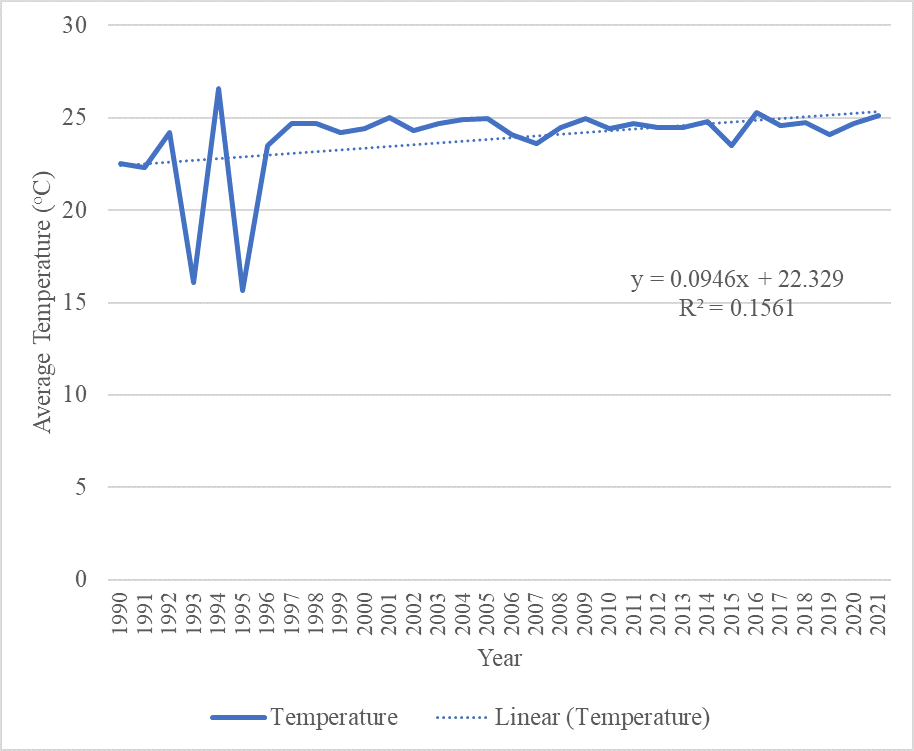
\includegraphics[width=0.9\textwidth]{images/trend_avg_temp.png}
\end{figure}

As shown in Figure~\ref{fig:trend_avg_temp}, the results indicate that between 1990 and 2020, the average temperature showed a minor positive trend, averaging 0.0946 degrees Celsius each year, with 15.61\% of the variability explained by the linear trend \( y = 0.0946x + 22.329 \). Aligning with findings from \parencite{regmiCROPYIELDRESPONSE2019} where  The average maximum temperature ranges from 26 to 31 with standard deviation of less than one and average minimum temperature ranges from 15 to 20 degrees Celsius again with standard deviation of less than one showing almost no change on its trend value. In contrast  \parencite{puriSpatialTemporalVariations2024} reported seasonal variability in temperature trends over a 60-year period in the Koshi Basin, detecting an overall slightly insignificant cooling trend. Similarly, \parencite{risalImpactClimateChange2022} observed a linear but modest increasing trend in temperature for the Banke region using the $NOAA\_RegCM4$ model. However, the analysis revealed less variability in the linear trend, with a decrease in average and maximum temperatures, while minimum temperatures showed an increasing trend. \parencite{dawadiImpactClimateChange2022} reported that while the annual maximum temperature exhibited an increasing trend (0.01°C per year), the overall annual temperature showed a decreasing trend (0.04°C per year).
The positive trend observed in our study may be attributed to global warming, which could have profound impacts on crop production. Rising temperatures influence crop growth, development, and yield, while also altering pest and disease distribution, potentially affecting agricultural productivity.

\begin{figure}[H]
    \centering
    \caption{Average Sunshine Hour since 1990 to 2021} 
    \label{fig:trend_avg_sunshine_hour}
    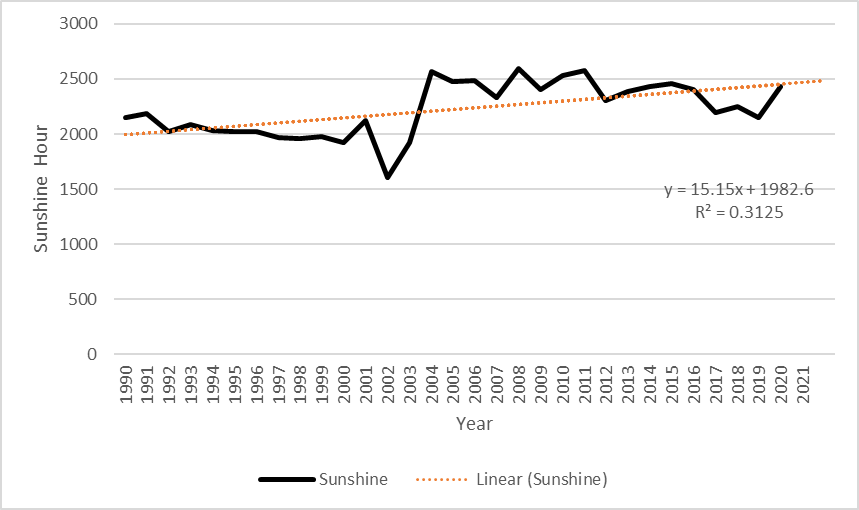
\includegraphics[width=0.9\textwidth]{images/trend_avg_sunshine_hour.png}
\end{figure}

The average sunlight hours from 1990 to 2020 exhibited a positive trend, increasing by 15.15 hours per year with an intercept of 1982.6, as shown in the linear trend analysis. The R-squared value (0.3125) indicates that the trend explains 31.25\% of the variability (Figure~\ref{fig:trend_avg_sunshine_hour}). This increase in sunlight hours in Banke may be influenced by weather variations, land-use changes, and climate variability, potentially driven by local and global climate change.


\begin{figure}[H]
    \centering
    \caption{Accumulated Rainfall since 1990 to 2021} 
    \label{fig:trend_accumulated_rainfall}
    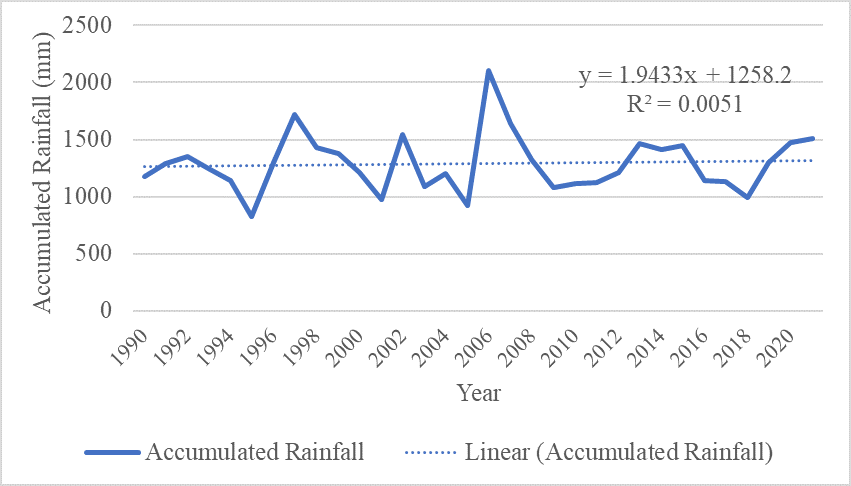
\includegraphics[width=0.9\textwidth]{images/trend_accumulated_rainfall.png}
\end{figure}


Figure~\ref{fig:trend_accumulated_rainfall} shows a slight positive trend in accumulated rainfall, represented by the equation $y=1.9433x + 1258.2$, indicating an annual increase of approximately 1.94 mm per year. This rise in rainfall in Banke, Nepal, may be influenced by local weather patterns, air circulation, land-use changes, and the broader effects of climate change. Similar to study by \parencite{poudelRelationshipsClimateVariability2016} in Lamjung District a mountainous region in Nepal, revealing heterogeneous precipitation trends, with two stations showing increasing precipitation and one showing a decreasing trend, likely influenced by the complex interplay of monsoon and westerly wind systems across the varied topography, while temperature analysis indicated a consistent warming trend, with an average increase of 0.07 degrees Celsius.
According to the \parencite{regmiCROPYIELDRESPONSE2019}, the average annual precipitation in Banke over the past 37 years is approximately 1395 mm, with values ranging from 868 mm to 2173 mm per year. The high standard deviation (over 338 mm) suggests significant variability in annual rainfall patterns. 
Rainfall patterns fluctuate annually, showing a lower degree of predictability. While there is an increasing trend in summer rainfall, winter rainfall is on the decline \parencite{maharjanEffectClimateVariables2013}.
\parencite{manandharAdaptingCroppingSystems2011} observed a diminishing trend in precipitation at the meteorological station at Bhairahawa Airport, along with highly irregular rainfall patterns in the region. Furthermore, although an analysis of temperature data indicates a marginal increase, the t-test results do not show any statistically significant trend.

\subsection{Yield and Climate Variables}
In this study to find the relationship between crop yield and climate variables, a correlation analysis was conducted between crop yield and key climate variables, including sunshine hours, accumulated rainfall, and average temperature, followed by a linear regression analysis.

% Correlation Table
\begin{table}[htbp]
    \centering
    \caption{Correlation Table between Yield and Climate Variables}
    \resizebox{\textwidth}{!}{ % Resize table to fit within text width
    \begin{tabular}{@{}lccc@{}}
        \toprule
        & \textbf{Sunshine Hours} & \textbf{Accumulated Rainfall (mm)} & \textbf{Average Temperature (°C)} \\
        \midrule
        \textbf{Yield (mt/ha)} & 0.417* & -0.074 & 0.287 \\
        \textbf{(p-value)} & 0.017 & 0.686 & 0.112 \\
        \bottomrule
    \end{tabular}
    }
\end{table}

% Linear Regression Model Summary
\begin{table}[htbp]
    \centering
    \caption{Linear Regression Model Summary for Yield and Climate Data}
    \label{tab:reg_summary_climate_yield}
    \begin{tabular}{@{}lc@{}}
        \toprule
        \textbf{Dep. Variable} & Yield \\
        \textbf{Adjusted R-squared} & 0.161 \\
        \textbf{Significance (p-value)} & 0.048 \\
        \textbf{F-statistic} & 2.981 \\
        \textbf{R-squared} & 0.242 \\
        \bottomrule
    \end{tabular}
\end{table}

% Regression Coefficient Table
\begin{table}[htbp]
    \centering
    \caption{Regression Coefficients for Yield and Climate Data}
    \label{tab:reg_coef_climate_yield}
    \resizebox{\textwidth}{!}{ % Resize table to fit within text width
    \begin{tabular}{@{}lccccll@{}}
        \toprule
        \multirow{2}{*}{\textbf{Model}} & \multicolumn{2}{c}{\textbf{Unstandardized Coefficients}} & \textbf{Standardized} & \multirow{2}{*}{\textbf{t}} & \multirow{2}{*}{\textbf{Sig}} \\
        \cmidrule{2-3}
        & \textbf{B} & \textbf{Std. Error} & \textbf{Beta} & & \\
        \midrule
        \textbf{(Constant)} & -99.061 & 903.331 & - & -0.110 & 0.913 \\
        \textbf{Sunshine} & 0.670 & 0.291 & 0.391 & 2.306 & 0.029 \\
        \textbf{Accumulated Rainfall} & -0.279 & 0.279 & -0.168 & -0.999 & 0.326 \\
        \textbf{Average Temperature} & 43.825 & 32.148 & 0.232 & 1.363 & 0.184 \\
        \bottomrule
    \end{tabular}
    }
\end{table}





Table~\ref{tab:reg_coef_climate_yield} presents the correlation between crop yield and key climate variables: sunshine hours, accumulated rainfall, and average temperature.  The results indicate that sunshine hours have a significant positive correlation with crop yield $(r=0.417,p=0.017)$, suggesting that increased solar exposure enhances crop productivity. In contrast, accumulated rainfall exhibits a weak negative correlation $(r=-0.074,p=0.686)$, implying that rainfall variability does not have a statistically significant effect on crop yield. Average temperature shows a moderate positive correlation with yield $(r=0.287,p=0.112)$; however, this relationship is not statistically significant. These findings suggest that sunshine hours play a more critical role in influencing crop yield than rainfall or temperature variations.

The linear regression model (Table~\ref{tab:reg_summary_climate_yield}), which includes sunshine hours, accumulated rainfall, and average temperature as predictor variables, explains 24.2\% of the variation** in crop yield $(R^2 = 0.242)$. After adjusting for the number of predictors, the adjusted $(R^2) $value is 0.161, indicating moderate explanatory power. However, \parencite{maharjanEffectClimateVariables2013} found that multivariate regression analysis indicate that the model can explain variations in the yields of food crops, ranging from 40\% for paddy to only 2\% for barley. Despite this, the regression findings in the current study show few significant relationships between crop yield and climate variables.

The model suggests that while climate variables contribute to variations in crop yield, additional factors may also play a role. The regression equation derived from the analysis is as follows:  

$
\text{Crop Yield} = \beta_0 + \beta_1 (\text{Sunshine Hours}) + \beta_2 (\text{Accumulated Rainfall}) + \beta_3 (\text{Average Temperature}) + \varepsilon
$

\begin{equation}
    \begin{split}
        \text{Crop Yield} &= -99.061 + 0.670 \times \text{Sunshine} \\
        &\quad - 0.279 \times \text{Accumulated Rainfall} \\
        &\quad + 43.825 \times \text{Average Temperature}
    \end{split}
\end{equation}

The regression analysis presented in Table~\ref{reg_coef_climate_yield} highlights the differential influence of climate variables on crop yield. Sunshine hours exhibit a statistically significant positive effect on yield $(\beta = 0.391, p = 0.029)$, confirming that increased solar exposure enhances photosynthesis and improves crop productivity. In contrast, accumulated rainfall shows a negative but non-significant effect $(\beta = -0.168, p = 0.326)$, indicating that total precipitation levels alone do not significantly contribute to yield variations, in contrast \parencite{thapa-parajuliImpactClimateChange2016} ovserved positive correlation between precipitation and wheat yield. Average temperature demonstrates a positive but non-significant relationship $(\beta = 0.232, p = 0.184)$, suggesting that while temperature fluctuations influence crop growth, their effect is less direct compared to solar radiation.

The findings indicate that sunshine hours are the most influential climate variable affecting yield. The significant correlation and positive regression coefficient reinforce the role of solar radiation in enhancing plant photosynthesis, ultimately improving crop growth. This is consistent with prior studies conducted in Nepal and South Asia, which identified solar radiation as a key determinant of agricultural output \parencite{thapa-parajuliImpactClimateChange2016}.

Conversely, rainfall does not exhibit a statistically significant impact on yield, likely due to erratic precipitation patterns in the Banke district. Similar studies have reported that uneven rainfall distribution reduces soil moisture availability, adversely affecting crop health despite high total precipitation levels \parencite{regmiCROPYIELDRESPONSE2019}. \parencite{devkotaClimateChangeTrends2014} found that the mean temperature is rising slowly in the West Rapti River basin. Additionally, the region is frequently impacted by devastating floods and persistent rainfall, which cause extensive damage to standing crops. These findings suggest that rainfall variability, rather than total precipitation, plays a more critical role in yield determination.

\parencite{thapa-parajuliImpactClimateChange2016} found a complex relationship between temperature and wheat yields, indicating that initial temperature increases may enhance yields, particularly with an optimal minimum temperature of 20°C. However, they caution that this positive impact is limited by a threshold, beyond which further warming could have a detrimental effect on production. 
The moderate but non-significant relationship between temperature and yield suggests that temperature fluctuations influence crop growth but may also introduce counteracting effects. Higher temperatures can accelerate crop maturation but simultaneously increase evapotranspiration, leading to reduced soil moisture availability \parencite{shresthaFarmersPerceptionClimate2022}. This could explain why temperature, though positively correlated with yield, does not demonstrate strong statistical significance in the regression model.

\parencite{pokharauniversitynepalImpactClimateChange2020} found that a 1\% increase in rainfall improved rice yield by 0.45\%, whereas this study indicates a negative but weak relationship between rainfall and yield. The discrepancy may stem from variations in soil properties, irrigation availability, and crop types across regions. Similarly, \parencite{karkiStatusDriversFood2021} reported that sunshine hours significantly influenced wheat productivity, reinforcing this study’s conclusion that increased solar exposure enhances crop output. Furthermore, \parencite{risalImpactClimateChange2022} observed that temperature increases beyond optimal thresholds negatively impact yield, whereas this study does not find a strong negative effect, possibly due to regional climate adaptations. \parencite{dawadiImpactClimateChange2022} found that the overall analysis of maize, wheat, and potato production showed a significant increasing trend over the study period, while millet production exhibited an insignificant decreasing trend. \parencite{poudelRelationshipsClimateVariability2016} observed significant temporal fluctuations in crop yield trends, with an overall increasing pattern, likely driven by a combination of factors such as the impacts of climate change and the adoption of improved agricultural practices, including the introduction of new seed varieties, advanced agricultural technologies, enhanced irrigation systems, and refined crop management strategies.


\subsubsection{Climate Change Perception}


Table~\ref{tab:farmers_perception} highlights farmers' perceptions of climate change and its impacts. A unanimous agreement (\textit{index} = 1.00) confirms that farmers recognize climate change, yet awareness of specific temperature variations is low (\textit{index} = -0.88). Similarly, perceptions of climate change affecting agricultural productivity and untimely monsoons are weakly negative (\textit{index} = -0.88, -0.75), indicating uncertainty or reliance on adaptive measures. Conversely, moderate agreement exists regarding climate change’s role in pest outbreaks (0.28), crop abnormalities (0.275), and extreme events (0.155). Farmers also acknowledge observable evidence of climate change (\textit{index} = 0.47), though their understanding of its direct effects remains inconsistent.\parencite{dawadiImpactClimateChange2022} reported that nearly half of the respondents perceived an increase in temperature, while about 30\% disagreed with the notion of temperature change, and the remaining respondents reported a temperature decrease. Furthermore, a considerable number of respondents (62.86\%) were unaware of climate change and its impacts. Despite this, most respondents (62.86\%) exhibited lower-than-average perceptions of the effect of climate change on agricultural production. However, it is clear that the local population has indeed experienced the effects of climate change.

These findings suggest a need for targeted awareness programs to enhance farmers’ climate literacy, particularly on temperature fluctuations, rainfall variability, and pest dynamics. Strengthening localized adaptation strategies and access to climate information can help mitigate perceived uncertainties and improve agricultural resilience.


\begin{table}[htbp]
    \centering
    \caption{Farmer’s Perception on Climate Data}
    \label{tab:farmers_perception}
    \begin{tabular}{@{}lcc@{}}
        \toprule
        \textbf{Statement / Variables} & \textbf{Index} \\
        \midrule
        Climate change is happening & 1.00 \\
        Aware about the range of temperature experienced in locality & -0.88 \\
        Climate change affects agricultural productivity & -0.88 \\
        Effect of untimely monsoon on production & -0.75 \\
        Climate change affects the spread of pests and insects over crops & 0.28 \\
        Abnormalities in crops & 0.275 \\
        Extreme events in locality & 0.155 \\
        Evidence of climate change & 0.47 \\
        \bottomrule
    \end{tabular}
    \vspace{0.5cm}

    \textit{*Higher the index, stronger the perception.} \\
    \textit{Frequency of agreement/approval: +1, Frequency of disagreement/disapproval: -1, Frequency of don't know/absent: 0.}
\end{table}

\subsubsection{agriculture and Food Scenarios}
Table~\ref{tab:agriculture_food_scenario} presents key characteristics of the agricultural and food security scenario. The results indicate that mixed farming and crop diversification are rare, with 97.8\% of farmers practicing monoculture. Despite this, food production is largely sufficient, as 92.5\% report adequate yields, and only 7.5\% experience food shortages.

Food security appears stable, with 97\% of households not facing deficits, and 99.3\% reporting no undernutrition. Additionally, 97.8\% maintain food stocks, mainly sourced from their own production (95.5\%). However, institutional support for agriculture is minimal, with only 4.5\% receiving assistance.

The dominance of monoculture farming raises concerns about long-term sustainability, given climate uncertainties. While food availability is currently high, reliance on single-crop systems may increase vulnerability to climate shocks. Strengthening institutional support and promoting diversified farming practices could enhance resilience and long-term food security.

\begin{table}[htbp]
    \centering
    \caption{Agricultural and Food Scenario Characteristics}
    \label{tab:agriculture_food_scenario}
    \begin{tabular}{@{}lcc@{}}
        \toprule
        \textbf{Characteristics} & \textbf{Variables} & \textbf{Percentage} \\
        \midrule
        Mixed Farming & Yes & 2.2 \\
                     & No & 97.8 \\
        Crop Combination & Yes & 2.2 \\
                         & No & 97.8 \\
        Food Production & Enough & 92.5 \\
                        & Not Enough & 7.5 \\
        Food Deficit & Purchase from the market & 3.0 \\
                     & Not Deficit & 97.0 \\
        Undernutrition & No & 99.3 \\
                       & Yes & 0.7 \\
        Food Stock Present or Absent & Yes, Present & 97.8 \\
                                     & No, Absent & 2.2 \\
        Sources & Own Production & 95.5 \\
                & Markets & 4.5 \\
        Institutional Support & Yes & 4.5 \\
                              & No & 95.5 \\
        \bottomrule
    \end{tabular}
\end{table}

\subsubsection{Crop Calendar}
Table~\ref{tab:crop_calendar} highlights shifts in sowing and harvesting times for major crops over the past five years, primarily due to irregular monsoons and climate variability. Paddy cultivation, which previously started in mid-June, has been delayed to early August, with a corresponding shift in harvesting to November. Similar trends are observed for wheat, mustard, lentils, and pigeon pea, with delays in both sowing and harvesting periods. In similar vain \parencite{bhattaraiImpactClimateChange2021} reported that Nepalese farmers, who rely heavily on the timing, frequency, duration, and intensity of rainfall for crop cultivation, are being forced to alter their cropping patterns due to climate change

These changes indicate that farmers are adapting to unpredictable rainfall and shifting climatic patterns. However, no significant alterations are noted for seasonal vegetables and fruits, suggesting that perennial crops may be less affected by climate variability. The adjustments in the crop calendar reflect farmers' strategies to cope with environmental uncertainties, emphasizing the need for climate-resilient agricultural practices and improved water management to mitigate risks associated with shifting weather patterns.



\begin{table}[htbp]
    \centering
    \caption{Crop Calendar Based on Major Changes in Cropping Time}
    \label{tab:crop_calendar}
    \renewcommand{\arraystretch}{1.2} % Increase row height for better readability
    \setlength{\arrayrulewidth}{0.8pt} % Adjust border thickness
    \resizebox{\textwidth}{!}{  
        \begin{tabular}{|l|c|c|c|c|l|}
            \hline
            \textbf{Crop} & \multicolumn{2}{|c|}{\textbf{Before 5 Years}} & \multicolumn{2}{|c|}{\textbf{Recent Time (After 5 Years)}} & \textbf{Reason} \\
            \hline
            & \textbf{Sowing Month} & \textbf{Harvesting Month} & \textbf{Sowing Month} & \textbf{Harvesting Month} &  \\
            \hline
            Paddy & June (3rd week) & September (1st week) & August (1st week) & November (Mid-week) & Irregular Monsoon / Climatic Shift \\
            \hline
            Wheat & December (1st week) & April (Last week) & January (Mid-week) & April (2nd week) & Climatic Shift \\
            \hline
            Mustard & November (Mid-week) & April (Mid-week) & November (3rd week) & March (2nd week) & Climatic Shift \\
            \hline
            Lentils & October (3rd week) & March (3rd week) & December (1st week) & April (Last week) & Climatic Shift \\
            \hline
            Pigeon Pea & June (Last week) & January (2nd week) & July (3rd week) & February (2nd week) & Climatic Shift \\
            \hline
            Vegetables & All months & All months & All months & All months & No Change \\
            \hline
            Fruits & All months & All months & All months & All months & No Change \\
            \hline
        \end{tabular}
    }
    \vspace{0.5cm}
    
    \textit{Source: Questionnaire survey conducted in the study area.}
    \end{table}
    

\subsection{Irrigation}
\subsubsection{irrigation Status}



The irrigation status in the study area is largely dependent on seasonal rainfall, with 93.3\% of land relying on rain-fed irrigation, while only 26.9\% has access to year-round irrigation (Table~\ref{tab:irrigation_data}). The predominant irrigation sources include a combination of groundwater, canal, drainage ponds, and rainfall, with 59\% of farmers depending on groundwater and drainage ponds. 

Gravity-fed surface irrigation, utilizing both flood and furrow techniques, is universally practiced across the region. Although 48.5\% of farmers rely on artificial irrigation, 38.1\% still depend on natural water sources, highlighting limited infrastructure for controlled irrigation. 

Despite the strong reliance on rainfed agriculture, respondents did not report significant irrigation issues, suggesting either sufficient seasonal water availability or adaptation to existing climatic conditions. However, the high dependence on monsoon rainfall makes agricultural productivity vulnerable to climate variability, underscoring the need for improved irrigation infrastructure and water storage solutions to enhance year-round water security.




\begin{table}[htbp]
    \centering
    \caption{Frequency Table for Land and Irrigation Data of Survey}
    \label{tab:irrigation_data}
    \begin{tabular}{@{}lcc@{}}
        \toprule
        \textbf{Characteristics} & \textbf{Variables} & \textbf{Percentage} \\
        \midrule
        \multirow{4}{*}{Irrigation Source} & Ground water + Canal irrigation + Rainfall & 23.9 \\
        & Ground water + Drainage Pond + Rainfall & 59.0 \\
        & Ground water + Rainfall & 1.5 \\
        & All & 15.7 \\
        \midrule
        \multirow{2}{*}{Land Quality Irrigation} & Khet & 73.1 \\
        & Upland and Khet & 26.9 \\
        \midrule
        \multirow{3}{*}{Irrigation Type} & Natural & 38.1 \\
        & Artificial & 48.5 \\
        & Both & 13.4 \\
        \midrule
        \multirow{2}{*}{Irrigation Category} & Year-round irrigation (whole year) & 6.7 \\
        & Rainfed Irrigation (monsoon) & 93.3 \\
        \midrule
        \multirow{2}{*}{Season of Availability} & All Season & 26.9 \\
        & Monsoon & 73.1 \\
        \midrule
        Irrigation Technique & Gravity-fed surface (flood and furrow) & 100.0 \\
        \bottomrule
    \end{tabular}
\end{table}

\subsubsection{Irrigation and yield}


The t-test results, as shown in Table~\ref{tab:t_test_irrigation}, compare the crop yield between two irrigation methods: year-round irrigation and rainfed irrigation in Janaki Rural Municipality. The findings indicate a significant difference in mean crop yield between the two irrigation methods.

\begin{table}[htbp]
    \centering
    \caption{t-test of Between-Subjects Effects}
    \label{tab:t_test_irrigation}
    \begin{tabular}{@{}l c c c c c c@{}}
        \toprule
        & \multicolumn{2}{c}{\textbf{Year-Round Irrigation}} & \multicolumn{2}{c}{\textbf{Rainfed Irrigation}} & \multicolumn{2}{c}{t(132), p} \\
        \cmidrule(lr){2-3} \cmidrule(lr){4-5}
        \textbf{Yield (kg/ha)} & \textbf{Mean} & \textbf{SD} & \textbf{Mean} & \textbf{SD} & \textbf{t} & \textbf{p} \\
        \midrule
        Crop Yield & 7868.63 & 3756.38 & 5450.43 & 2505.86 & 2.696 & 0.008 \\
        \bottomrule
    \end{tabular}
\end{table}

For year-round irrigation, the mean crop yield was 7868.63 kg/ha, with a standard deviation of 3756.38, while for rainfed irrigation, the mean crop yield was 5450.43 kg/ha, with a standard deviation of 2505.86. The t-test analysis produced a t-value of 2.696 and a p-value of 0.008, which is statistically significant at the 0.05 level. This suggests that year-round irrigation leads to significantly higher crop yields compared to rainfed irrigation. According to \parencite{mallaClimateChangeIts2009} that rainfed wheat productivity is likely to be more vulnerable in the Terai than in the mid-hills under a climate change scenario.

This result aligns with similar studies that have shown the benefits of consistent irrigation on crop yields. The difference in yield underscores the importance of irrigation infrastructure and access to reliable water sources for improving crop productivity. It also highlights the vulnerability of rainfed agriculture to climate variability, emphasizing the need for more sustainable and resilient irrigation practices to safeguard food security in the region.


